\documentclass[11pt,a4paper]{article}
\usepackage[utf8]{inputenc}
\usepackage[T1]{fontenc}
\usepackage{amsfonts}
\usepackage[french]{babel}
\frenchbsetup{StandardLists=true} % à inclure si on utilise \usepackage[francais]{babel}
\usepackage{enumitem}
\usepackage{amssymb}
\usepackage{amsmath}
\usepackage[left=2cm,right=2cm,top=2cm,bottom=2cm]{geometry}
\usepackage{multirow}
\usepackage[dvipsnames]{xcolor}

\usepackage[T1]{fontenc}
\usepackage{fouriernc}
\usepackage{graphicx}

\usepackage{setspace}
\singlespacing

\usepackage{pstricks}
\usepackage{xkeyval}
\usepackage{pst-labo}


\usepackage{multicol}
\usepackage{caption}
\usepackage{fancyhdr}
\pagestyle{fancy}
\renewcommand\headrulewidth{1pt}
\fancyhead[L]{Lycée Denis Diderot }
\fancyhead[R]{Classe de Terminale}
\setcounter{page}{10}\fancyfoot[C]{page \thepage}
\fancyfoot[R]{Année 2025 2026}
\fancyfoot[L]{Alexis RUIZ}
\usepackage{multirow,tabularx,booktabs}
\newcommand{\cadreblanc}[1]{%
\medskip\framebox[\linewidth][c]{%
\rule{0mm}{#1mm}}\par
\medskip}

\usepackage{awesomebox}
\setlength{\aweboxvskip}{0mm}
\usepackage{pifont}
\usepackage{chemmacros}
\chemsetup{modules=all}

\renewcommand{\arraystretch}{2}
\newcommand*\acocher{\quitvmode{\fboxsep0pt \fboxrule0.8pt \fbox{\vrule height1.8ex depth.1ex width0pt \vrule height0pt depth0pt width1.9ex }}}

\newcommand{\defproblem}{\awesomebox[black]{2pt}{\rotatebox{90}{\large{\textbf{Problématique}}}}{black}}
\newcommand{\defconclusion}{\awesomebox[black]{2pt}{\rotatebox{90}{\Large{\textbf{Conclusion}}}}{black}}
\newcommand{\defbox}{\awesomebox[black]{2pt}{
\includegraphics[scale=0.5]{images/appel exam.png}}{black}}


\frenchbsetup{StandardLists=true}
\begin{document}



\center \LARGE{TP3 - Acide et métaux}
\\[0,3cm]

\normalsize

\hrule\
\\[0,2cm]

\flushleft \textbf{NOM :\\
Prénom:\\[0,2cm]
}
\hrule\
\\[0,2cm]

\textbf{Expérience \ding{202} :} Dans un tube à essais verser quelques millilitres de solution d'acide chlorhydrique (\ch{HCl})  et introduire une tournure de cuivre. \\[3mm]

\fbox{
\begin{minipage}{17cm}{
\textbf{Noter vos observations : }\\
\vspace{1cm}
}

\end{minipage}
}
\vspace{5mm}



\begin{figure}[h]
{\begin{minipage}{0.2\textwidth}
\begin{center}
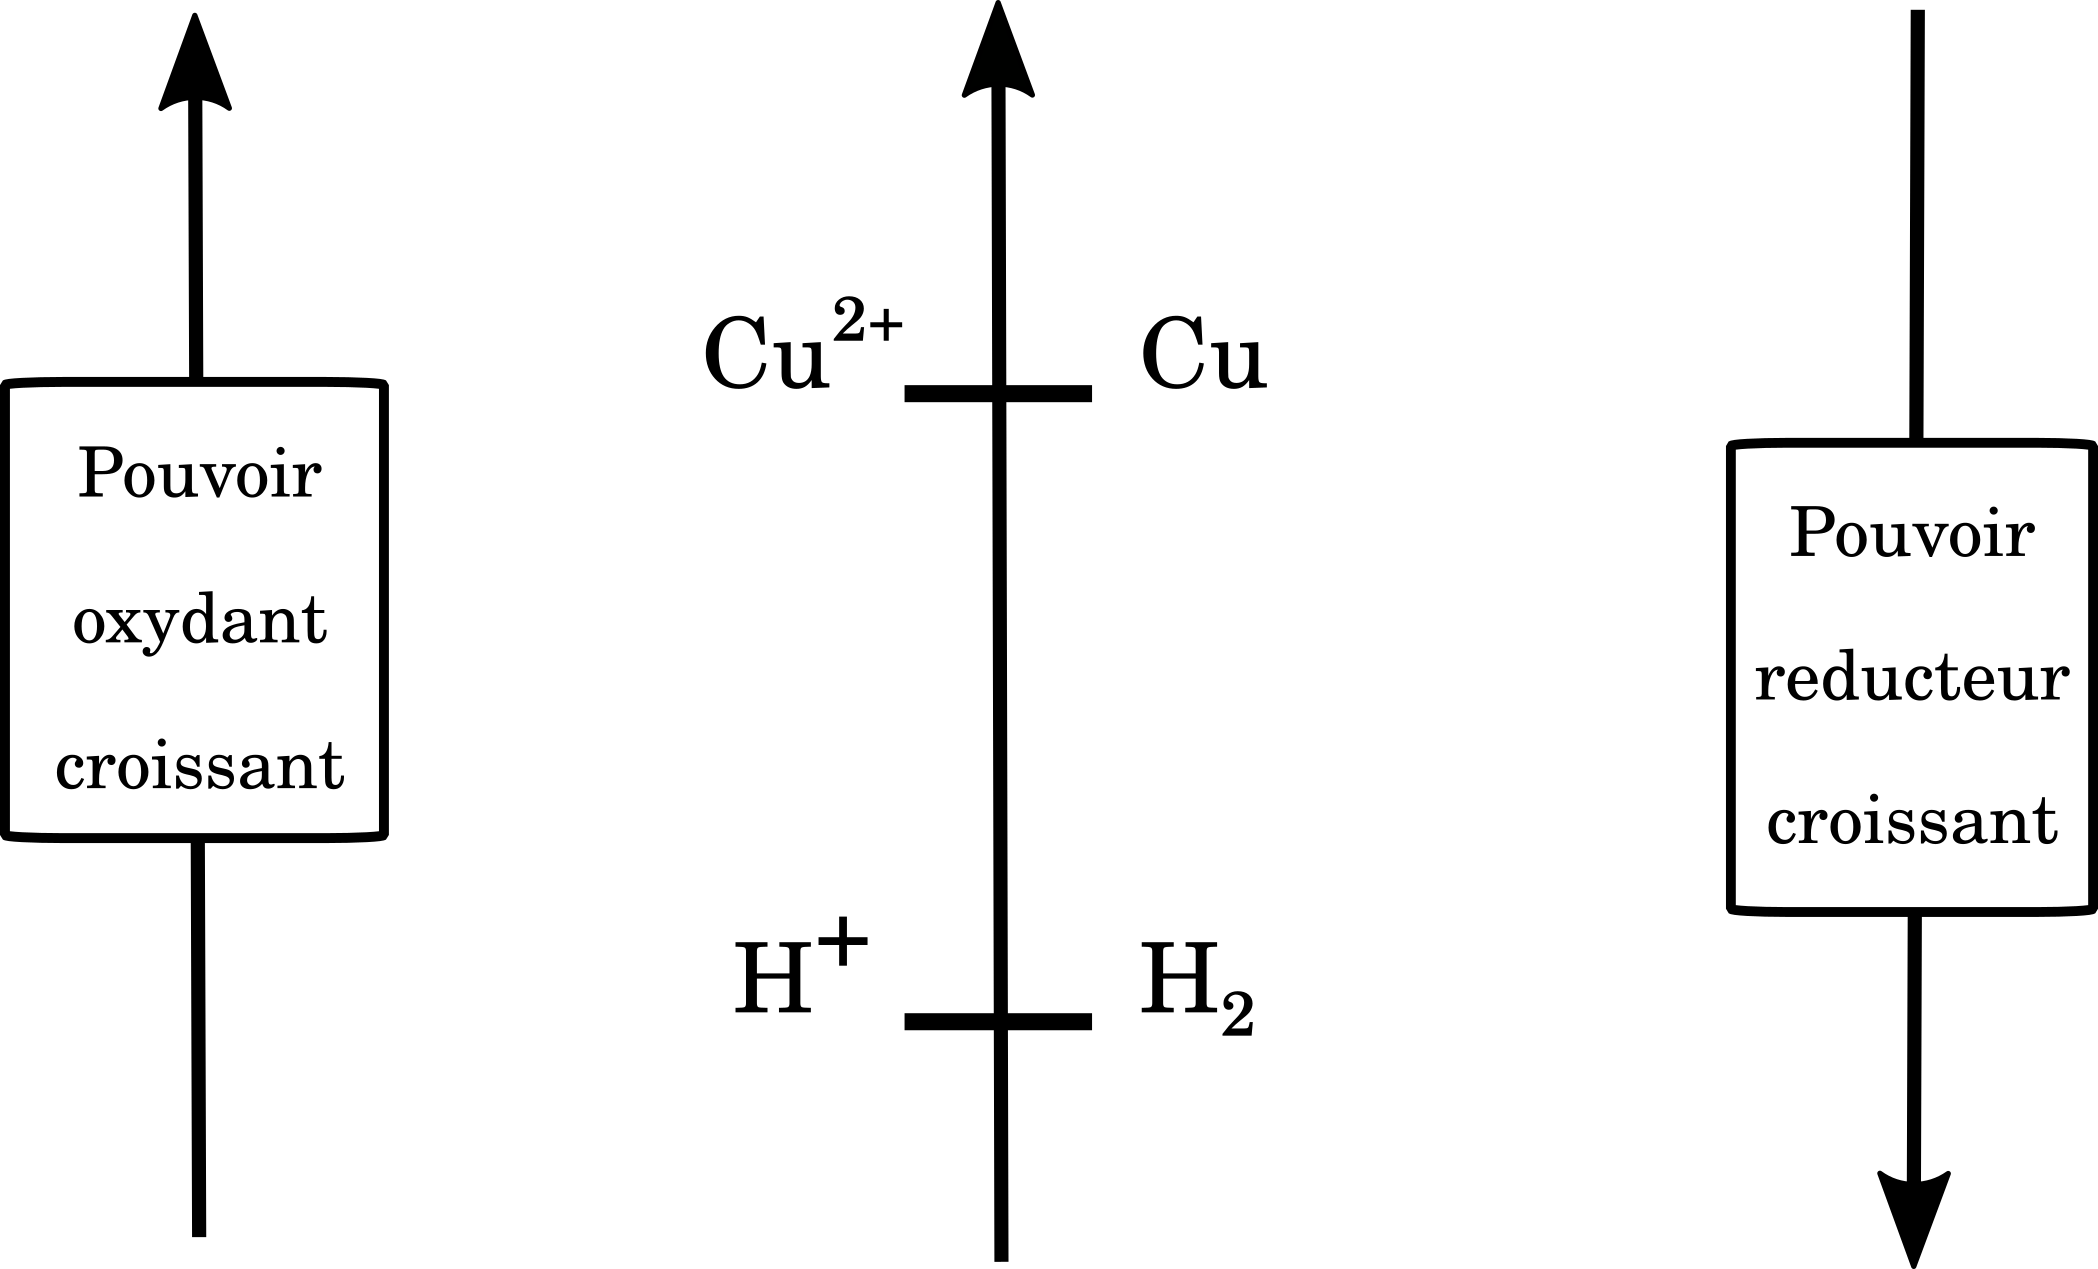
\includegraphics[scale=0.20]{images/classification 2 elements h et cu.png} 
\end{center}
\end{minipage}}~~~~
\begin{minipage}{0.79\textwidth}
En utilisant la classification des couples rédox ci-contre, justifier vos observations. \\
\textit{Aide : la solution d'acide chlorhydrique (\ch{HCl}) contient des ions hydrogène (\ch{H\pch[]})}\\

\vspace{5mm}
\dotfill

\vspace{10mm}

\dotfill

\end{minipage}
\end{figure}

\textbf{Expérience \ding{203} :} Dans un tube à essais introduire de la poudre de fer (\ch{Fe}) puis verser quelques millilitres de solution d'acide chlorhydrique (\ch{HCl}) \\[3mm]

\begin{figure}[h]
\begin{minipage}{0.2\textwidth}
\begin{center}
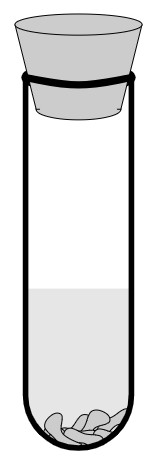
\includegraphics[scale=0.25]{images/Tube acide.jpg} 
\end{center}
\end{minipage}~~~~
\fbox{\begin{minipage}{0.79\textwidth}
Notez vos observations. \\
\vspace{2 cm}


\end{minipage}}
\end{figure}

\defbox{\fbox{
\begin{minipage}{14cm}{
Appeler le professeur pour effectuer le test à la flamme. Si une détonation se produit, vous êtes en présence de dihydrogène (\ch{H_2})}

\end{minipage}
}}
\vspace{5mm}

Prélever , un peu de liquide et l'introduire dans un autre tube à essai. \\[1cm]

Ajouter quelques gouttes d'hydroxyde de sodium \ch{NaOH}. Décrire la couleur du précipité observé. \\
\cadreblanc {15}

\newpage

A l'aide du tableau d'identification des ions présents ci-dessous, identifier l'ion présent dans la solution, entourer sa formule chimique dans le tableau. 
\begin{center}
\fbox{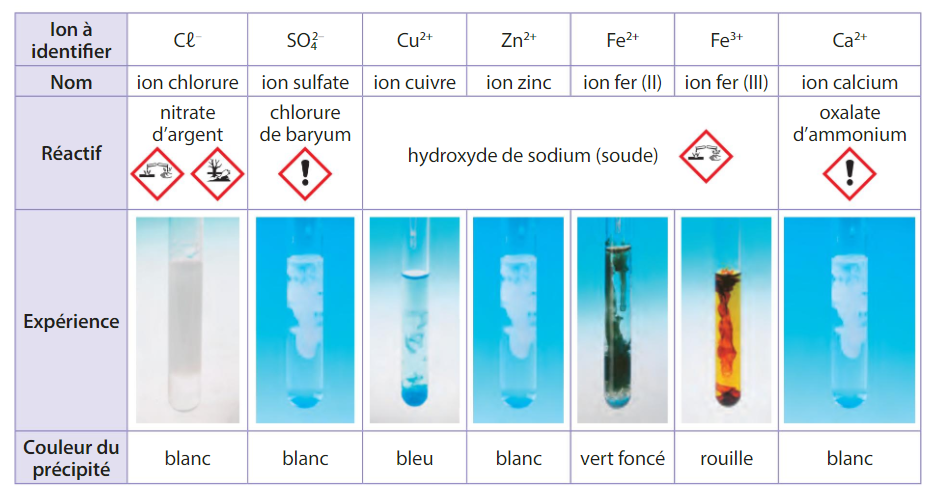
\includegraphics[scale=0.5]{images/tableau pp.png} }
\end{center}

\fbox{
\begin{minipage}{16.5cm}{
Écrire les demi-équations de réaction puis l'équation bilan. }
\vspace{3cm}
\end{minipage}
}
\vspace{5mm}


\defbox{\fbox{
\begin{minipage}{14.2cm}{
Verser la solution et le reste du métal dans le bêcher de récupération puis nettoyer votre matériel }

\end{minipage}
}

}
\vfill 

\hline
\vfill 

\textbf{Conclusion : } Placer les couples \ch{H\pch[]} / \ch{H_2} ; \ch{Cu\pch[2]} / \ch{Cu}  et \ch{Fe\pch[2]} / \ch{Fe}  dans l'échelle électrochimique ci-dessous :  

\vspace{5mm}
\begin{center}
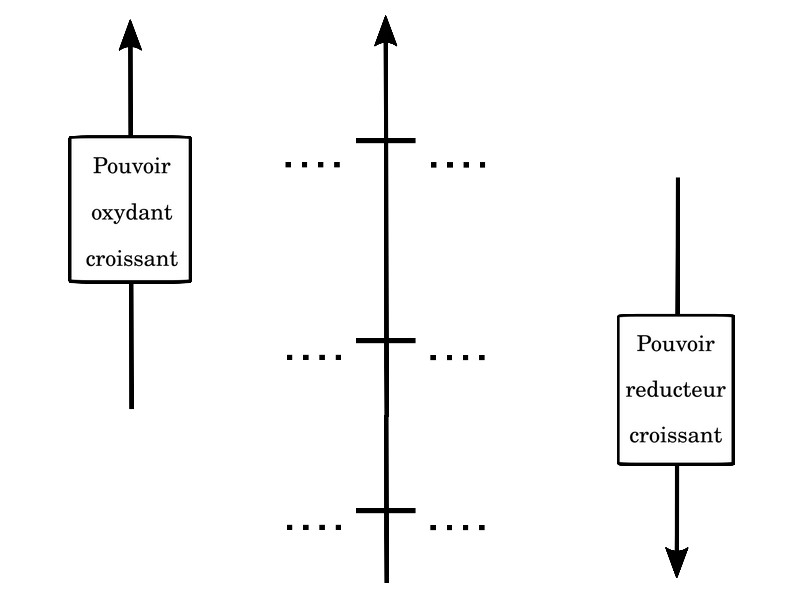
\includegraphics[scale=1.2]{images/Echelle 3 elements.jpg}
\end{center}

\vfill
\end{document}